\documentclass{beamer}
\setbeamertemplate{page number in head/foot}{}
\setbeamertemplate{theorems}[ams style]
% Use a modern theme
\usetheme{metropolis}
% Enable Swedish language support
\usepackage[swedish]{babel}
\usepackage[T1]{fontenc}
\usepackage[utf8]{inputenc}

\usepackage{graphicx}

\usepackage{amsthm}

\newtheorem{faktum}{Faktum}

%\usecolortheme{whale}

% Title page information
\title{En budget för tillväxt?}
\author{Karl Harmenberg}
\institute{\url{karlharmenberg.com}}
\date{14 oktober 2024}

\AtBeginSection[]{
  \begin{frame}
  \vfill
  \centering

    \usebeamerfont{title}\insertsectionhead\par%

  \vfill
  \end{frame}
}

\begin{document}

% Title slide
\frame{\titlepage}


% Table of contents
\begin{frame}{Översikt}
    \tableofcontents

    \bigskip

    Pythonkod för att reproducera alla resultat: \url{https://github.com/karlharmenberg/bnp2024}
\end{frame}



\section{Europeisk tillväxt}

\begin{frame}{Tillväxt i utvecklade länder}

	\begin{center}
        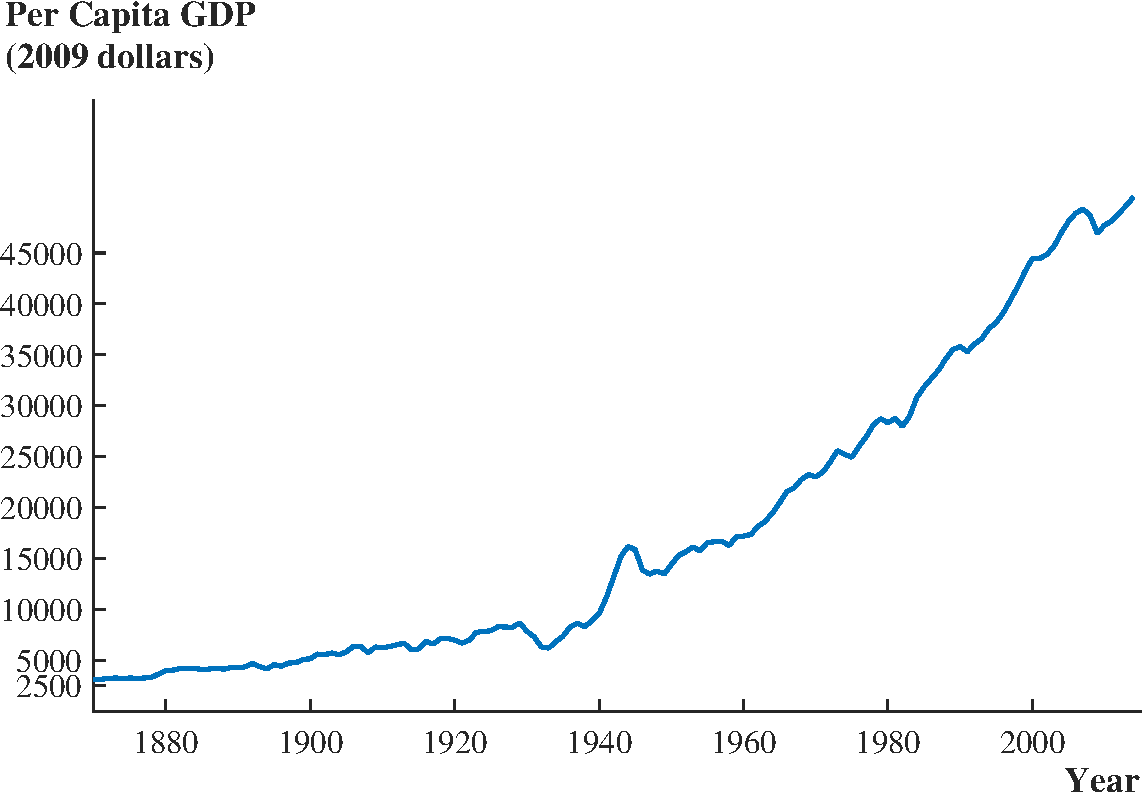
\includegraphics[scale=0.4]{figures/uspcgdp1-crop.pdf}

        Real BNP per capita, USA
    \end{center}

    \bigskip

    {\footnotesize\color{blue}\href{https://web.stanford.edu/~chadj/facts.pdf}{``The Facts of Economic Growth'' (Jones 2016)}}
\end{frame}

\begin{frame}{Tillväxt i utvecklade länder}

	\begin{center}
        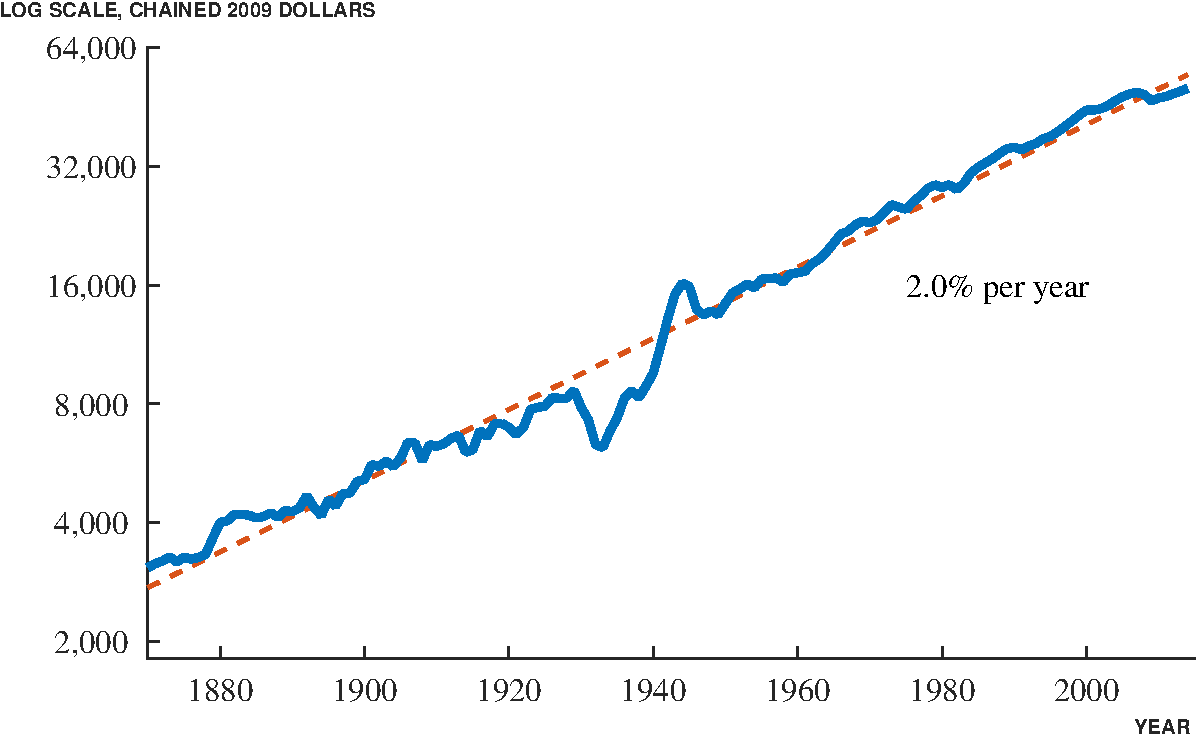
\includegraphics[scale=0.4]{figures/uspcgdp2-crop.pdf}

        Log(Real BNP per capita), USA
    \end{center}
    
    \bigskip

    {\footnotesize\color{blue}\href{https://web.stanford.edu/~chadj/facts.pdf}{``The Facts of Economic Growth'' (Jones 2016)}}
\end{frame}

\begin{frame}{Är två procent tillväxt en naturlag?}

    \begin{itemize}
        \item Nej, så klart inte. Tillväxt är ett modernt fenomen. Senaste tjugo åren har tillväxten varit betydligt lägre.
        \item Framtiden:
        \begin{itemize}
            \item Lägst hängande frukterna plockade?
            \item Teknologisk revolution med AI?
        \end{itemize}

        \bigskip

        \item Är hög BNP-tillväxt eftersträvansvärt?
        \begin{itemize}
            \item Målet är ett bra samhälle och förbättrad livskvalitet (samt ekologiskt hållbart). En del av ökat välstånd: mer fritid, inte minst som andel av livslängden.
            \item I praktiken: ökad produktivitet $\leadsto$ ökat välstånd.
        \end{itemize}
    \end{itemize}
    
\end{frame}

\begin{frame}{Europeisk tillväxt och amerikansk tillväxt}
    \begin{center}
        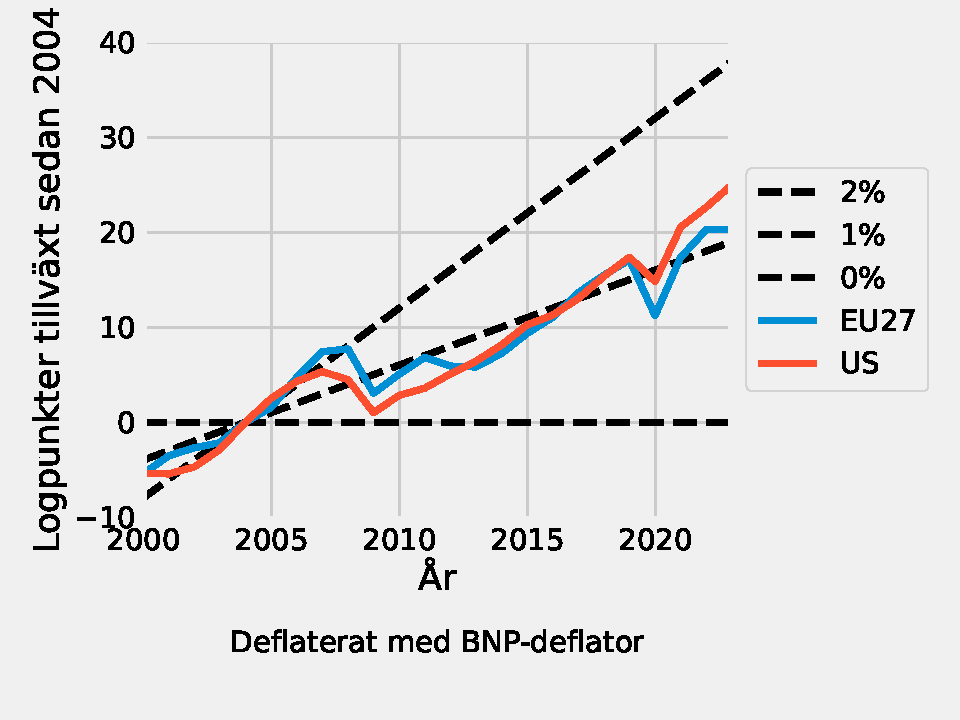
\includegraphics[width=0.7\textwidth]{figures/GDP_growth0_world.pdf}
    \end{center}

    \bigskip
    \footnotesize
    USA och Europa har haft (väldigt) liknande tillväxt.
\end{frame}

\begin{frame}{Draghirapporten}
    \begin{quote}
        ``Across different metrics, a wide gap in GDP has opened up between the EU and the US, driven mainly by a more pronounced slowdown in productivity growth in Europe. \\(p. 1)'' %Europe's households have paid the price in foregone living standards. On a per capita basis, real disposable income has grown almost twice as much in the US as in the EU since 2000.
    \end{quote}

    \bigskip

    \begin{itemize}
        \item Det här är fel.
        \item Sedan länge är BNP per capita högre i USA ($\approx 30\%$ PPP).
        \item Den högre \emph{tillväxten} i USA beror på befolkningstillväxt.\footnote{``The gap has widened less on per capita basis as the US has seen faster population growth /.../ in PPP terms, it has risen from 31\% in 2002 to 34\% today. (p. 8)''}
    \end{itemize}
\end{frame}

\begin{frame}{Europeisk tillväxt}
    \label{eu_growth}
    \begin{center}
        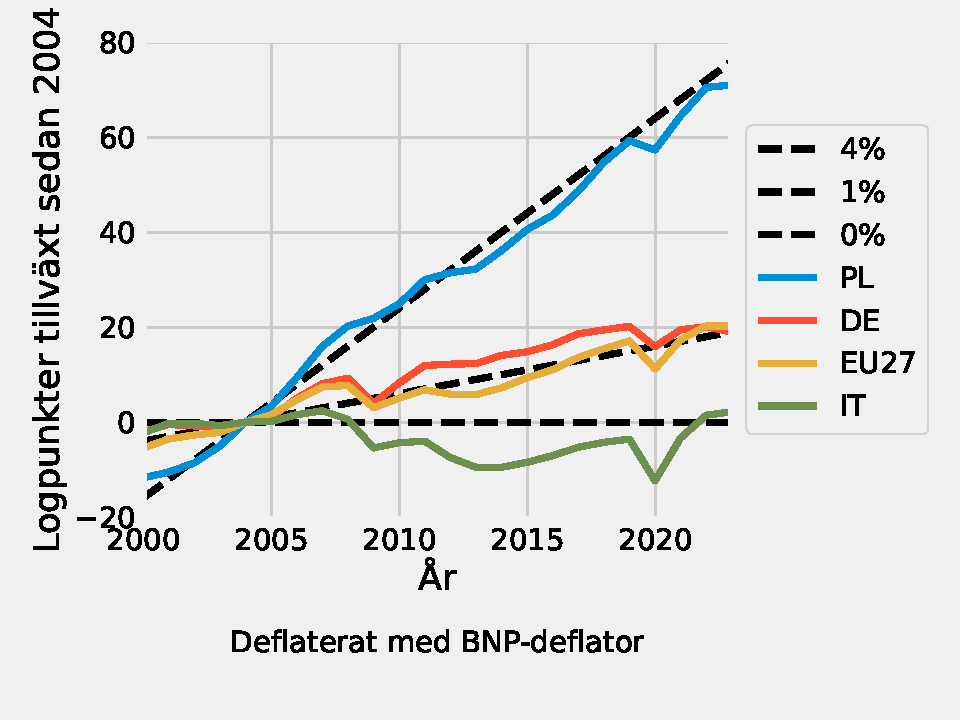
\includegraphics[width=0.7\textwidth]{figures/GDP_growth0_Europe.pdf}
    \end{center}
    \bigskip

    {\footnotesize Stora variationer inom Europa. \\ \color{blue}\href{https://cepr.org/voxeu/columns/eu-miracle-when-75-million-reached-high-income}{The EU Miracle: When 75 Million Reach High Income}} \\
    \hyperlink{communist}{\beamerbutton{Forna kommunistländer}}
    \hyperlink{pigs}{\beamerbutton{PIGS}}
\end{frame}

\begin{frame}{Fakta: USA och Europa}
    \begin{enumerate}
        \item USA och Västeuropa har haft en tvåprocentig tillväxt i BNP per capita de senaste hundra åren.
        \item De senaste tjugo åren har USA och Europa haft enprocentig tillväxt i BNP per capita.
        \item USA och Europa har haft väldigt lik tillväxt i BNP per capita de senaste tjugo åren.
        \item Tillväxten varierar stort inom Europa. Östeuropa har hög tillväxt, Sydeuropa låg tillväxt, och nordeuropeiska länder har haft en tillväxt nära medelvärdet.
    \end{enumerate}
\end{frame}

\section{Norsk tillväxt}
\begin{frame}{Norsk tillväxt sedan 2004}
    \begin{center}
        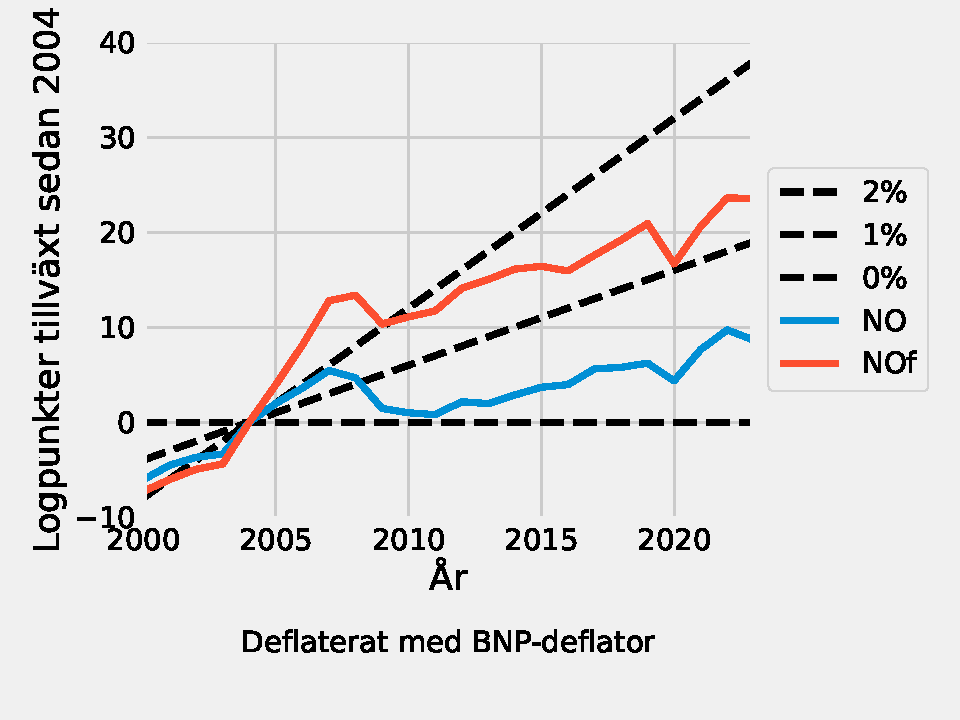
\includegraphics[width=0.7\textwidth]{figures/GDP_growth0_NO.pdf}
        \begin{itemize}
            \small
            \item NOf $=$ Fastlandsnorge
            \item Perspektivmeldingen 2021: 1,1 \% per år 2020-2060.
            \item Perspektivmeldingen 2024: 0,7 \% per år 2024-2060.
        \end{itemize}
    \end{center}
\end{frame}

\begin{frame}{Norsk tillväxt sedan 2004}
    \begin{center}
        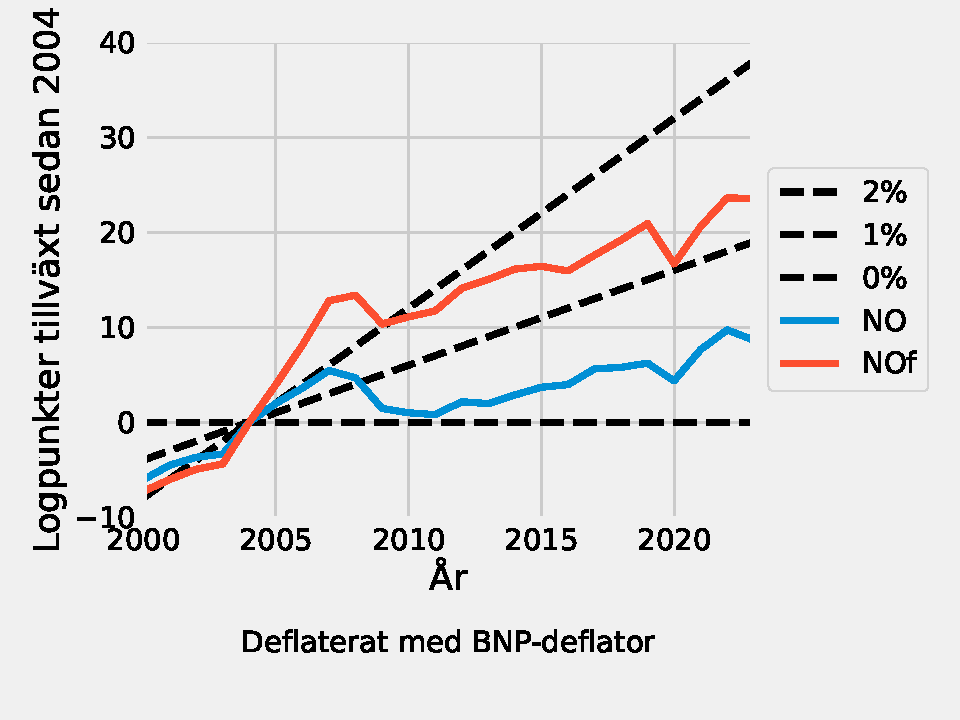
\includegraphics[width=0.7\textwidth]{figures/GDP_growth0_NO.pdf}
        \begin{itemize}
            \small
            \item Deflaterat med BNP-deflator $\sim$ fysisk produktivitet
            \begin{itemize}
                \item Alternativ: köpkraftsjusterat med KPI
                \item För andra länder, liten skillnad. För Norge: stor skillnad.
            \end{itemize}
        \end{itemize}
    \end{center}
\end{frame}

\begin{frame}{Norsk tillväxt sedan 2004}
    \begin{center}
        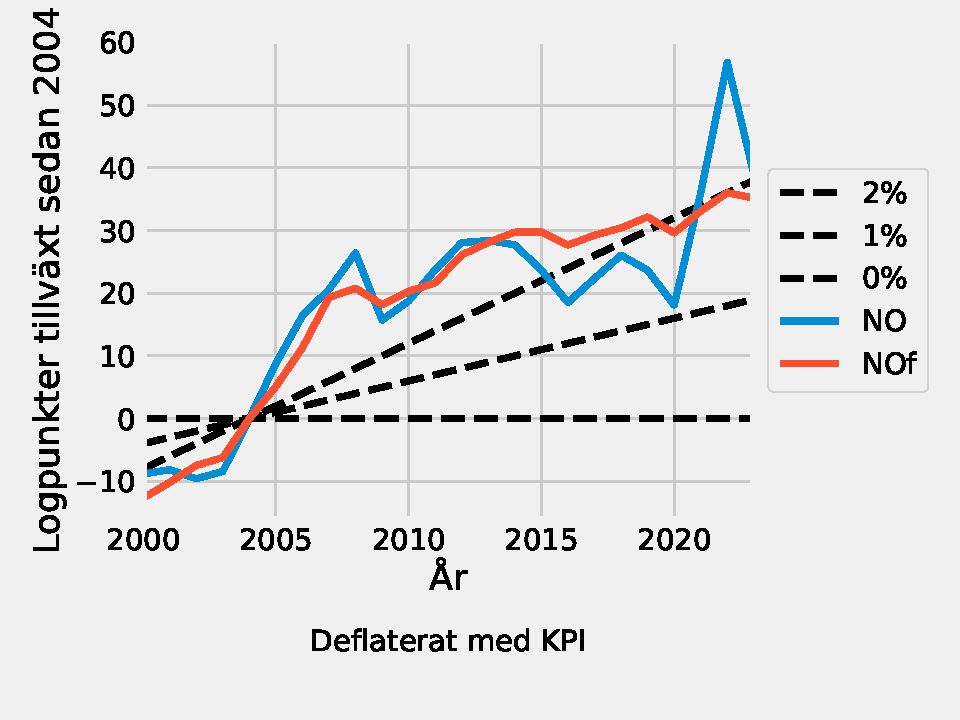
\includegraphics[width=0.7\textwidth]{figures/GDP_growth1_NO.pdf}
        \begin{itemize}
            \small
            \item Deflaterat med KPI $\sim$ köpkraft. Högre tillväxt än BNP-deflaterat pga högre priser på exportvaror  (olja).
            \item Liknande utveckling för Norge och Fastlandsnorge. 
            \begin{itemize}
                \item Hypotes: oljenära sektorer på fastlandet viktiga + ``rents''?
            \end{itemize}
        \end{itemize}
    \end{center}
\end{frame}

\begin{frame}{Norsk tillväxt i skandinaviskt sammanhang}

    \label{scandinavia_gdp}
    \begin{center}
        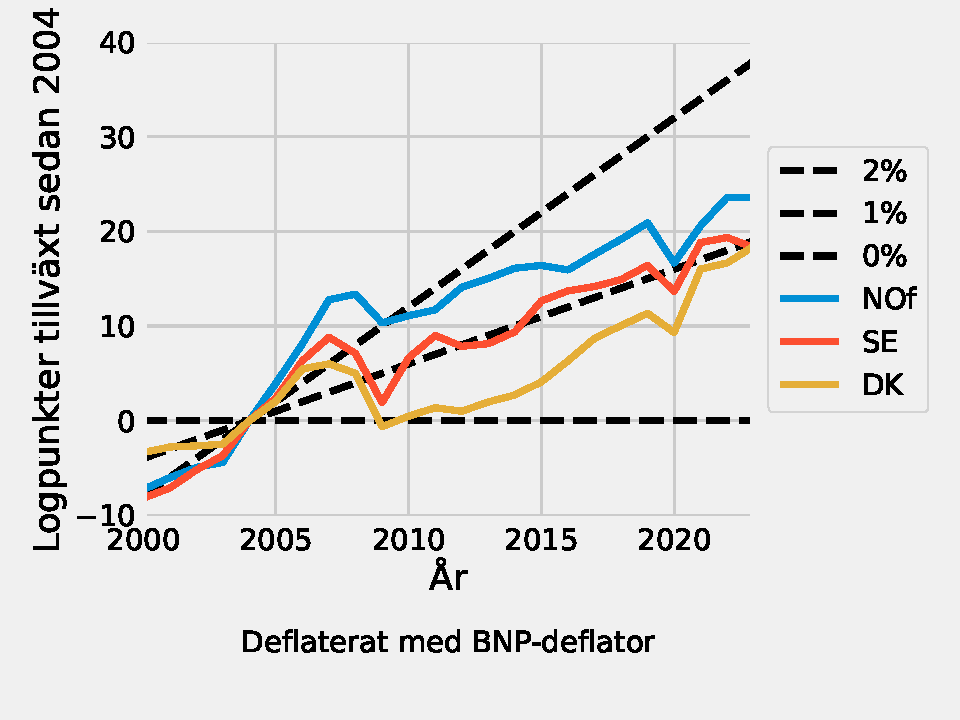
\includegraphics[width=0.7\textwidth]{figures/GDP_growth0_Scandinavia.pdf}
        \begin{itemize}
            \item Fastlandsnorge har samma tillväxt som Sverige och Danmark.
        \end{itemize}
    \end{center}

    \hyperlink{scandinavia_cpi}{\beamerbutton{Deflaterat med KPI}}
\end{frame}



\begin{frame}{Norsk tillväxt i europeiskt sammanhang}

    \label{europe_gdp}
    \begin{center}
        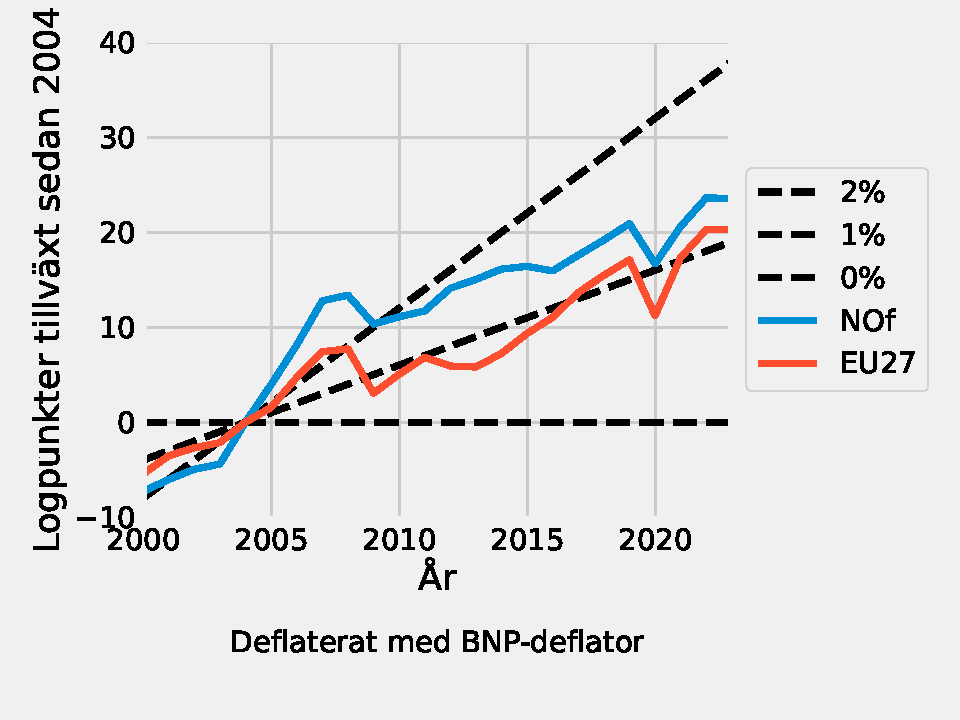
\includegraphics[width=0.7\textwidth]{figures/GDP_growth0_Europe_Norway.pdf}
    \end{center}

    \hyperlink{europe_cpi}{\beamerbutton{Deflaterat med KPI}}
\end{frame}

\begin{frame}{Fakta: Norge}

    \begin{enumerate}
        \item Fastlandsnorge har haft en tillväxt nära medelvärdet för Europa de senaste tjugo åren.
        \item Köpkraftsjusterad BNP per capita för Fastlandsnorge har haft en tvåprocentig tillväxt de senaste tjugo åren.
    \end{enumerate}

\end{frame}

\section{En budget för tillväxt?}



\begin{frame}{En budget för tillväxt?}
    
    \begin{itemize}
        \item Samma tillväxt i Europa, USA, Skandinavien och Norge de senaste tjugo åren.
        \begin{itemize}
            \item Politik spelar roll, se på Sydeuropa.
        \end{itemize}
        \item Viktigt: humankapital, innovation, kapital, företagande, attraktivt land att bo och verka i.
        \item Industripolitik?
        \begin{itemize}
            \item Viktigare än att välja vinnare är att avveckla misslyckade industrisatsningar.
        \end{itemize}
        \item Orealistiskt att ett litet land är världsledande på många fronter. Behöver inte vara det (geopolitik på europeisk nivå).
        \begin{itemize}
            \item Cuddly capitalism vs. cut-throat capitalism.
            \item Små talens lag: ha tur! (jmfr Danmark/Novo Nordisk/Ozempic)
        \end{itemize}
    \end{itemize}

\end{frame}

\begin{frame}
\Huge
\vfill
\begin{center}
    Takk!
\end{center}
\vfill
\end{frame}

\begin{frame}{Tillväxt i forna kommunistländer}
    \label{communist}
    \begin{center}
            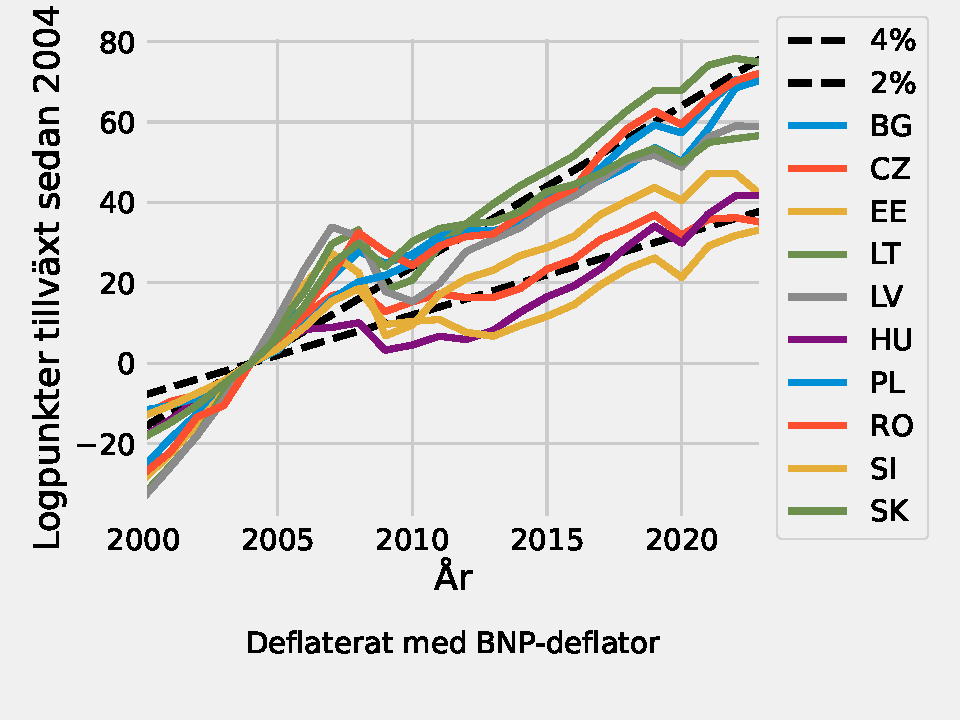
\includegraphics[width=0.7\textwidth]{figures/GDP_growth0_Europe_former_communist.pdf}
    \end{center}

    \bigskip
    \footnotesize
    Hög tillväxt bland forna kommunistländer.
    \hyperlink{eu_growth}{\beamerbutton{Tillbaka}}
\end{frame}

\begin{frame}{Tillväxt i ``PIGS''}
    \label{pigs}
    \begin{center}
        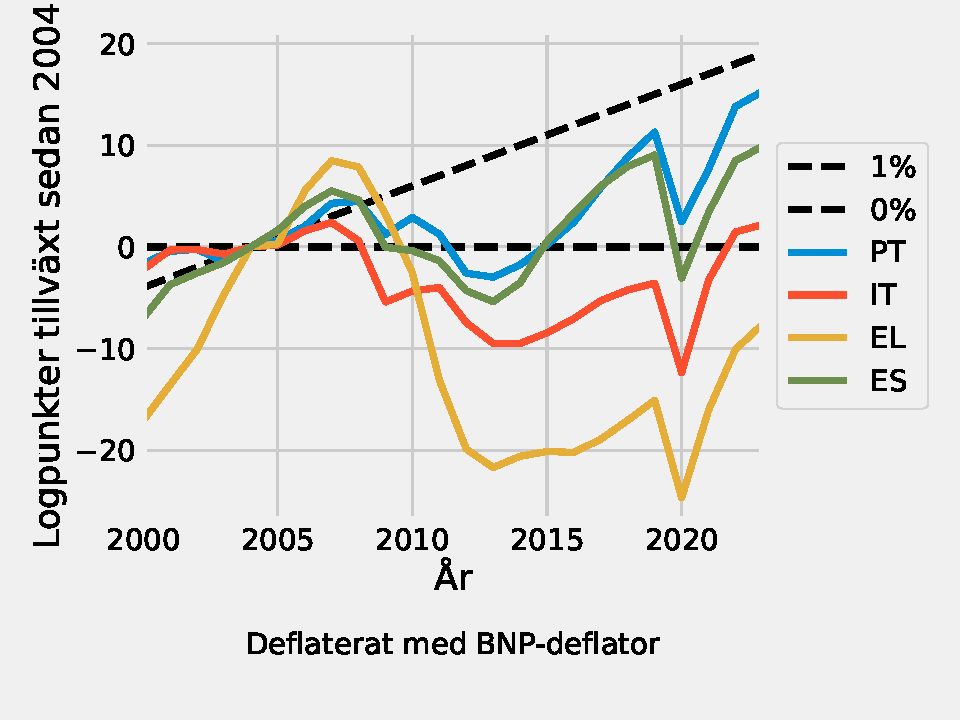
\includegraphics[width=0.7\textwidth]{figures/GDP_growth0_PIGS.pdf}
    \end{center}
    \bigskip
    \footnotesize
    Låg tillväxt i Sydeuropa.
    \hyperlink{eu_growth}{\beamerbutton{Tillbaka}}
\end{frame}

\begin{frame}{Norsk tillväxt i skandinaviskt sammanhang}
    \label{scandinavia_cpi}
    \begin{center}
        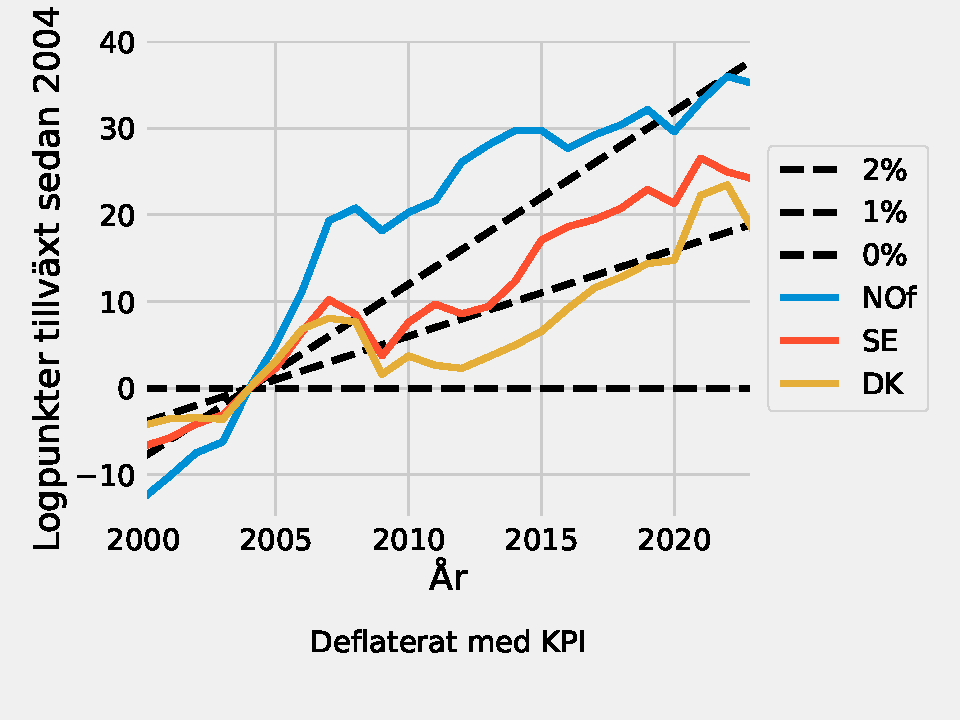
\includegraphics[width=0.7\textwidth]{figures/GDP_growth1_Scandinavia.pdf}
        \begin{itemize}
            \item Fastlandsnorge har samma starkare tillväxt än Sverige och Danmark, köpkraftsjusterat.
        \end{itemize}
    \end{center}

    \hyperlink{scandinavia_gdp}{\beamerbutton{Tillbaka}}
\end{frame}

\begin{frame}{Norsk tillväxt i europeiskt sammanhang}
    \label{europe_cpi}
    \begin{center}
        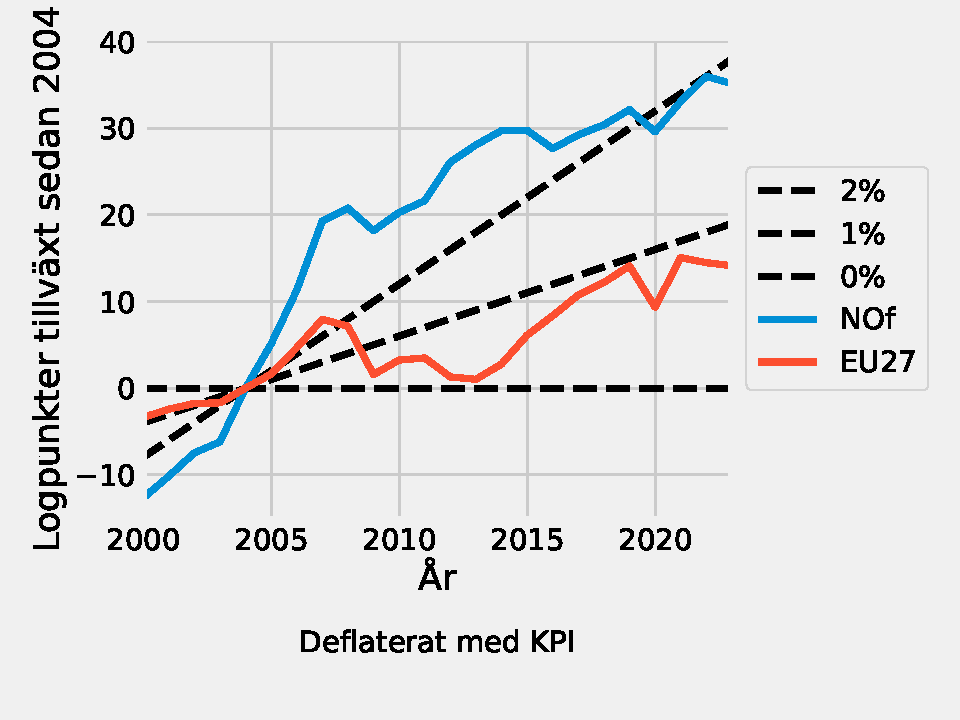
\includegraphics[width=0.7\textwidth]{figures/GDP_growth1_Europe_Norway.pdf}
    \end{center}
    \hyperlink{europe_gdp}{\beamerbutton{Tillbaka}}
\end{frame}

\end{document}
